\section{Research Methodology}
\label{sec:methodology}

The research work for this Thesis involves two distinct knowledge domains: law and ontology engineering. As such, distinct research methods were followed for the distinct stages of this research, in particular:

\begin{itemize}
    \item To analyse knowledge sources (Section \ref{sec:law_review})
    \item To review state of the art solutions to represent privacy terms in decentralised settings (Section \ref{sec:technical_review})
    \item To create and validate vocabularies (Section \ref{sec:ontology_engineering})
    \item To publish and archive research software (Section \ref{sec:code_preservation})
\end{itemize}

\subsection{Literature review}
\label{sec:literature_review}

In this Section, the methodology to analyse legal knowledge sources and review state of the art solutions to represent privacy terms in decentralised settings is introduced.

\subsubsection{Review of legal knowledge sources}
\label{sec:law_review}

The legal knowledge, upon which this research is based, is derived from the General Data Protection Regulation.
In particular, an analysis was made of Chapters III and IV (`Rights of the data subject' and `Controller and processor', respectively), where each article in both chapters was manually studied to search for interactions between the entities and the information that needs to be exchanged between them.

In addition to the text of the GDPR, the following sources were utilised or mentioned:

\begin{itemize}
    \item Guidelines and opinions published by EDPB\footnote{\url{https://edpb.europa.eu/} (accessed on 22 October 2023)}.
    \item Joint opinions and technical reports published by EDPS\footnote{\url{https://edps.europa.eu/} (accessed on 22 October 2023)}.
    \item Guidelines and opinions published by the Article 29 Data Protection Working Party (WP 29)\footnote{\url{https://ec.europa.eu/newsroom/article29/items/itemType/1360} (accessed on 22 October 2023)}.
    \item Other data-related legislation of the European Parliament and Council, in particular, the DGA, the eIDAS and its proposed amendment, and the EHDS proposal.
    \item Research publications in the personal data protection domain, in particular, related to the GDPR.
\end{itemize}

\subsubsection{Literature Review of Solid, Policy Languages and Data Protection Vocabularies}
\label{sec:technical_review}

Throughout the years different methodologies have been published for conducting a literature review~\citep{webster_analyzing_2002, kitchenham_systematic_2013} and, in particular, in 2019, a survey of distinct categories of methodologies, including guidance on how to execute and evaluate them, was published by~\cite{snyder_literature_2019}.
Three types of review methodologies are described, namely, systematic, semi-systematic, and integrative approaches. % TODO: \beatriz{add a description of each methodology type }
Also according to~\citeauthor{snyder_literature_2019}, the choice of the correct approach is related to the research questions, purpose, or style of the document being reviewed.

As such, an integrative approach~\citep{whittemore_integrative_2005} was used as it is the most appropriate for the objective of synthesising academic publications, in particular regarding the description and development of different policy languages and data protection vocabularies in a qualitative and quantitative manner, i.e., coverage of distinct personal data-related concepts and count of modelled concepts, respectively.
The same approach was taken to evaluate research on semantic-based personal datastores.
Moreover, the snowballing procedure~\citep{wohlin_guidelines_2014} was followed to search for relevant academic publications to be included in this Thesis, as well as other public documentation as it is advised by the integrative literature review approach.
Additional citation analysis research was performed using~\citeauthor{webster_analyzing_2002}'s backward and forward snowballing methodologies -- examine the reference list of the already identified publications to determine new documents that should be considered and select new research publications that cite the ones already being considered, respectively.

The collected publications were reviewed, evaluated, and, if relevant, included in the state of the art, according to the following criteria:

\begin{itemize}
\item Availability of a publication to review.
\item Only publications in English were considered.
\item Existence of online resources, e.g., ontology documentation or RDF/OWL specifications, was considered beneficial, as it allows for a better understanding and a quantitative evaluation of the reviewed solution.
\item Pre- and Post-GDPR works were considered.
\end{itemize}

\subsection{Ontology engineering}
\label{sec:ontology_engineering}

The Linked Open Terms (LOT)\footnote{More details regarding the methodology and the tools promoted by LOT are available at \url{https://lot.linkeddata.es/} (accessed on 14 June 2023).} methodology for the specification, implementation, publication, and maintenance of ontologies~\citep{poveda-villalon_lot_2022} was used for the development of the ontologies in this Thesis, as it is based on existing methodologies for the development of Semantic Web technologies and it is aligned with software development and research projects lifecycles.
Moreover, the~\cite{suarez-figueroa_neon_2012} methodology was used to define formal competency questions (CQ) and to collect the ontologies requirements, which are then consolidated in an Ontology Requirement Specification Document (ORSD).
Figure~\ref{fig:lot} presents a diagram of the main steps of the LOT methodology workflow, with a specific focus on the ontologies implementation phase.

\begin{figure}
    \centering
    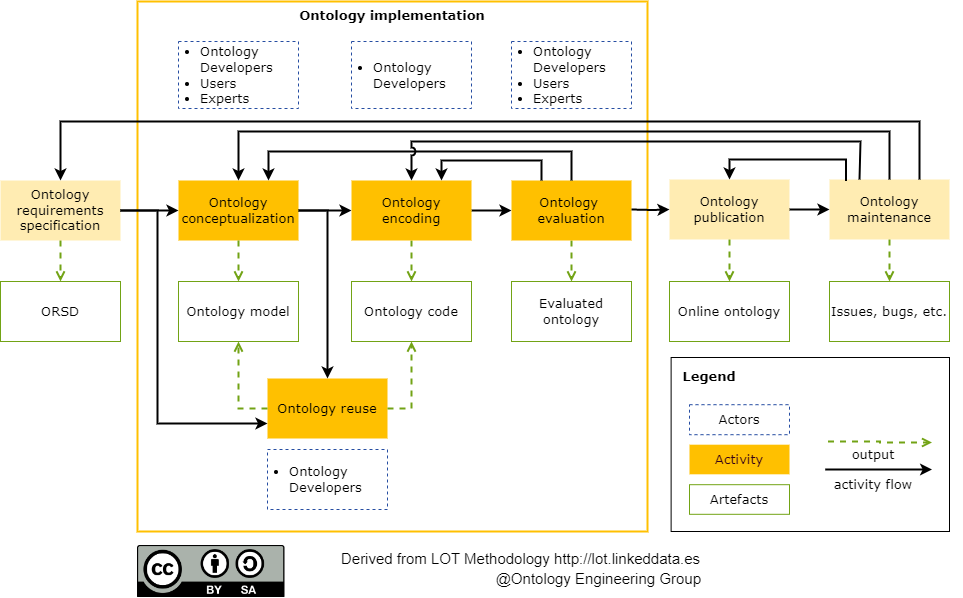
\includegraphics[width=\linewidth]{figures/chapter-3/LOT.png}
    \caption{Ontology development workflow based on the LOT methodology.}
    \label{fig:lot}
\end{figure}

Taking into account the requirements specified in the ontologies' ORSD, their first conceptualisations were then generated through a visualisation tool, the Chowlk Visual Notation tool\footnote{The Chowlk Converter tool and respective usage instructions are available at \url{https://chowlk.linkeddata.es/} (accessed on 14 June 2023).}~\citep{chavez-feria_chowlk_2022}, followed by feedback from experts. The generated conceptualisation diagrams were then used to generate the first version of the ontologies encoding as a Turtle file.
Furthermore, after the generation of the first version of the ontologies, the created terms were evaluated against a set of use case scenarios and using SPARQL queries.
From this evaluation, if necessary, new concepts were added to the ontologies, and the ORSDs were also updated accordingly.
The ontologies were also evaluated by using the OntOlogy Pitfall Scanner (OOPS!)\footnote{The OOPS! tool is available at \url{https://oops.linkeddata.es/} (accessed on 14 June 2023).}~\citep{poveda-villalon_oops_2014} to detect common errors in ontology development, such as missing domain or range properties or missing annotations, and using FOOPS!\footnote{The FOOPS! tool is available at \url{https://w3id.org/foops} (accessed on 30 November 2023).}, the Ontology Pitfall Scanner to ensure ontology alignment with the Findable, Accessible, Interoperable and Reusable (FAIR) principles~\citep{garijo_foops_2021}.
As a final evaluation, ontologies classes and properties and, in particular, their definitions were reviewed by legal and technical experts and, when applicable, connected with the relevant legal rules, guidelines, and other literature.

The ontologies are published using the \url{w3id.org}, ``Permanent Identifiers for the Web'', service\footnote{This service is run by the W3C Permanent Identifier Community Group (\url{https://www.w3.org/community/perma-id/}, accessed on 22 October 2023).}.
This service provides a secure and permanent re-direction and content negotiation service that serves both human-readable documentation and a machine-readable file from the same URI.
The source code is hosted on GitHub\footnote{\url{https://github.com/} (accessed on 22 October 2023)} and version control is done using Git\footnote{\url{https://git-scm.com/} (accessed on 22 October 2023)}.

% TODO: mention SHACL validation + SPARQL for CQs}

\subsection{Publication and archival of research software}
\label{sec:code_preservation}

Recently, the scientific community has also been discussing extending FAIR data practices to research software~\citep{martinez_top_2019,gruenpeter_d44_2024}.
Extending such practices to software implies the inclusion of rich metadata, in machine and human-readable format, and unique persistent identifiers for software to be findable and accessible.
In terms of interoperability and reusability, software must include clear documentation and reuse instructions, as well as use common standards and platforms.
As such, the following best practices, adopted from the aforementioned guidelines, are followed to ensure the FAIR publication and preservation of research software in this Thesis:

\begin{enumerate}
    \item Description of the software is included in the README.md file of the software repository. 
    \item Software is archived in a software registry, i.e., Zenodo.
    \item Software has a persistent identifier such as Digital Object Identifier (DOI) and/or a \url{w3id.org}.
    \item Software is downloadable.
    \item Software follows a semantic versioning scheme.
    \item Software requirements are listed in the software repository.
    \item Software installation instructions are included in the README.md file of the software repository.
    \item Software usage instructions are included in the README.md file of the software repository.
    \item The software repository has a license.
    \item The software repository provides instructions on how to cite it.
    \item The software repository includes metadata including programming language, creation date, keywords, and releases.
\end{enumerate}

Moreover, the source code of the developed research software is hosted on GitHub and version control is done using Git.